%% These sections describes the design and implementation of the chosen sensors.

\section{Sensors} \label{sensors}
To implement the MPPT it's necessary to measure the output voltage and current of the PV-module. These measurements will be obtained by implementing a voltage and current sensor. A second voltage sensor will be implemented to measure the output voltage of the DC/DC coverter, for possible future use. 

To protect the RT-Box, it has been chosen to fully isolate it from the power stage of the converter. To do so, the sensors will have to include isolation between input and output.  

%%% Voltage sensors %%%
\subsection{Input voltage sensor} \label{voltage_sensors}
The voltage sensor selected is ACPL-C870 \cite{voltage_sensor}. This sensor includes optical isolation amplifiers, which makes it well suited for isolated voltage sensing. The amplifier includes unity gain $1V/V$ amplification, with an accuracy at $\pm 3 \%$. Figure \ref{fig:voltage_sensors_placement} shows the placement of the two voltage sensors, where $V_{in}$ and $V_{out}$ are the input and output sensor respectively. 

\begin{figure}[htbp]
	\begin{center}
		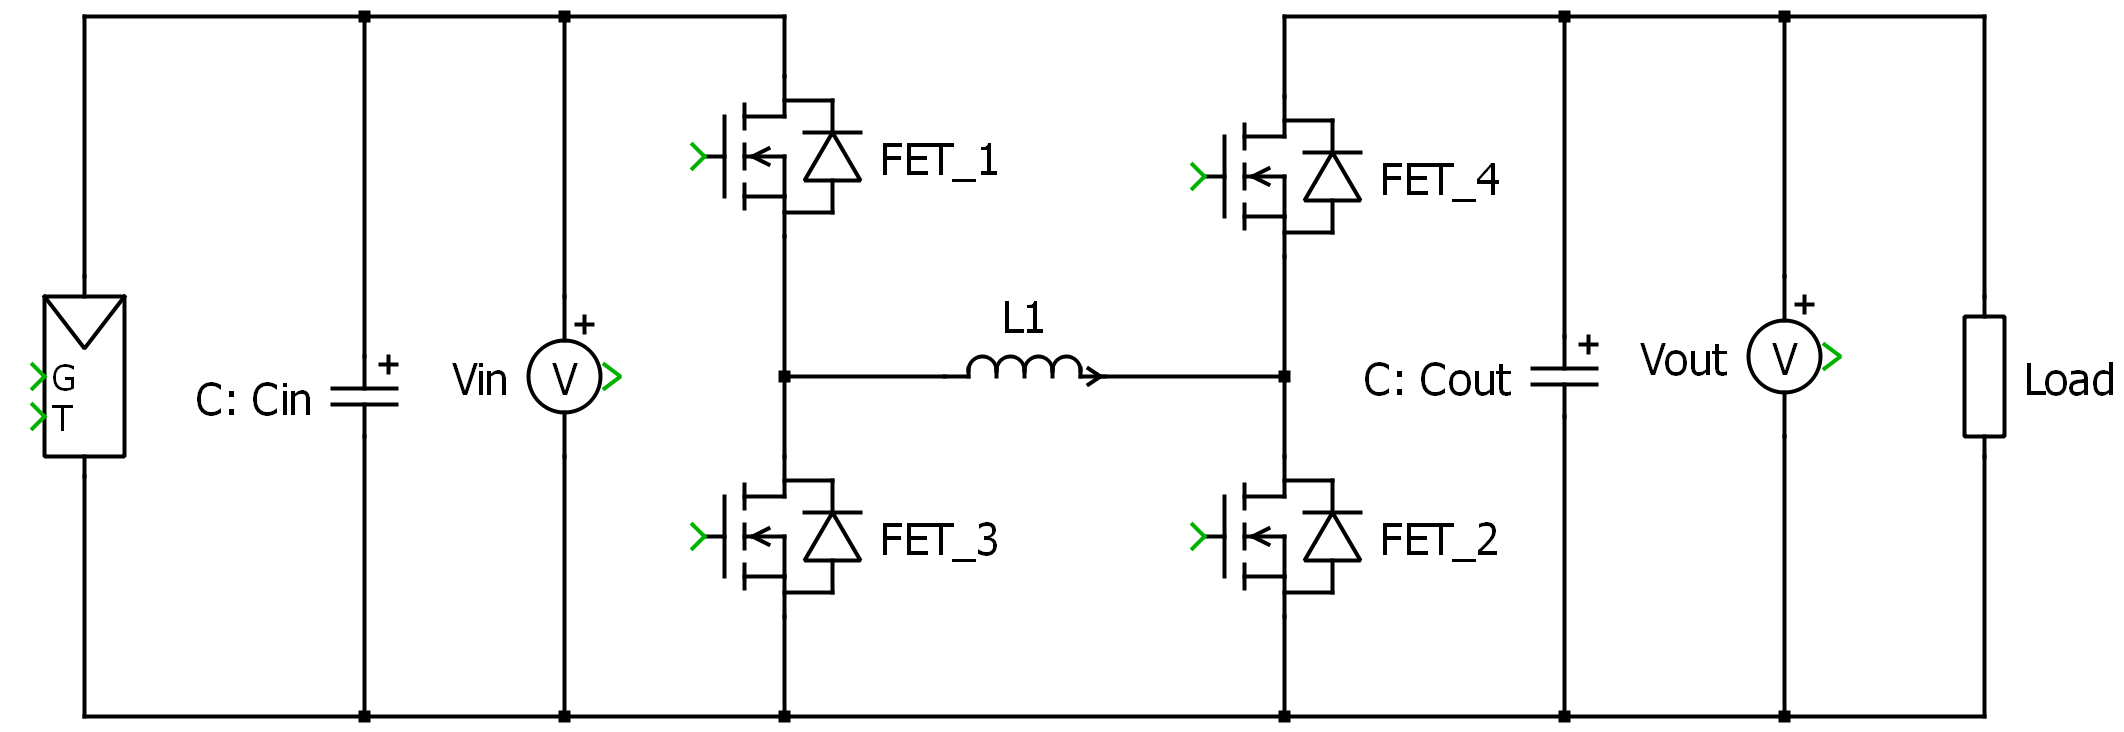
\includegraphics[width=0.7\linewidth]{../Pictures/P1/Sensors/voltage_sensors_placement.PNG}
		\caption{Voltage sensors placement}
		\label{fig:voltage_sensors_placement}
	\end{center}
\end{figure} 

\subsubsection{Voltage divider}
The input voltage at the voltage sensor is recommended to be in the range of $0V-2V$. To divide the measured voltage into that range, a voltage divider will be implemented. 

The maximum output voltage of the PV-module is the open-circuit voltage at $45.2V$. To achieve a safety margin and to make the converter adaptable to other types of PV-modules, $50V$ has been selected. The current flow in the voltage divider has been set at $1mA$, to secure a insignificant power loss. The resistors can be calculated with the following equations:
\begin{equation} \label{voltage_divider_R17_in}
	R_{17} = \frac{V_{in,max}-V_{out}}{I} = \frac{50V-2V}{1mA} = 48k\Omega
\end{equation}

\begin{equation} \label{voltage_divider_R18_in}
	V_{out} = V_{in,max} \cdot \frac{R_{18}}{R_{17}+R_{18}} \Rightarrow 2V = 50V \cdot \frac{R_{18}}{48k\Omega+R_{18}}
\end{equation}
\begin{center}
	$R_{18} = 1.958k\Omega$
\end{center}

To achieve these resistor values $R_{17} = 47k\Omega$ and $R_{18} = 2k\Omega$ have been chosen. 

\subsubsection{Filtering} \label{voltage_sensor_filter}
For a stable MPPT control, the measured voltage must have a very low ripple. To ensure this, a low-pass RC filter with a corner frequency at $500Hz$, will be placed between the voltage divider and the sensor. The resistor of the filter will be $R_1$ in the voltage divider. The capacitor will calculated as followed in equation \ref{voltage_sensor_in_filter_cap}:
\begin{equation} \label{voltage_sensor_in_filter_cap}
	C_{17} = \frac{1}{2\pi \cdot f_c \cdot R_{17}} = \frac{1}{2 \pi \cdot 500Hz \cdot 47k\Omega} = 6.7nF
\end{equation}

To achieve the capacitance $C_{17} = 6.6nF$ has been chosen. 

\subsubsection{Amplification} \label{voltage_sensor_amplification}
The input range of the ADC in the RT-Box is $0V-5V$. To take advantage of the entire range an amplifier will be implemented. The output of the voltage sensor is differential with an offset at $1.23V$. Therefore a differential amplifier will be implemented using a LMC6484 quad operational amplifier \cite{sensor_opamp}. By using a quad amplifier, the same IC can be used for the output voltage sensor and the current sensor.

The resistors of the differential amplifier will be sized with equation \ref{voltage_sensor_gain}.
\begin{equation} \label{voltage_sensor_gain}
	V_{out} = \frac{R_{22}}{R_{20}} \cdot (V_2-V_1)
\end{equation}

Where $V_2-V_1$ is the difference between the output pins of the voltage sensor. With unity gain in the voltage sensor, the maximum difference at the output will be $2V$. This should correspond to the maximum input voltage of the ADC at $5V$. $R_1$ is selected to be $11k\Omega$. The resistor $R_{22}$ is now calculated using equation \ref{voltage_sensor_gain}.
\begin{equation}
	5V = \frac{R_{22}}{11k\Omega} \cdot 2V
\end{equation}
\begin{center}
	$R_{22} = 27.5k\Omega$
\end{center}
To achieve the value of $R_{22}$ it's rounded to be $27k\Omega$. Furthermore $R_{19} = R_{20}$ and $R_{21} = R_{22}$, to get a balanced differential amplifier.

\subsubsection{The circuit}
The circuit regarding the input voltage measurement is shown at figure \ref{fig:input_voltage_sensor_circuit}. $V_{in}$ is the measured voltage from the PV-module. The points $OA1_+$ and $OA1_-$ are connected to the non-inverting and inverting input of the amplifier respectively. $OA1_{out}$ is connected to the output of the amplifier. $C_{15}$ and $C_{16}$ are decoupling capacitors for the two supply voltages. 

\begin{figure}[H]
	\begin{center}
		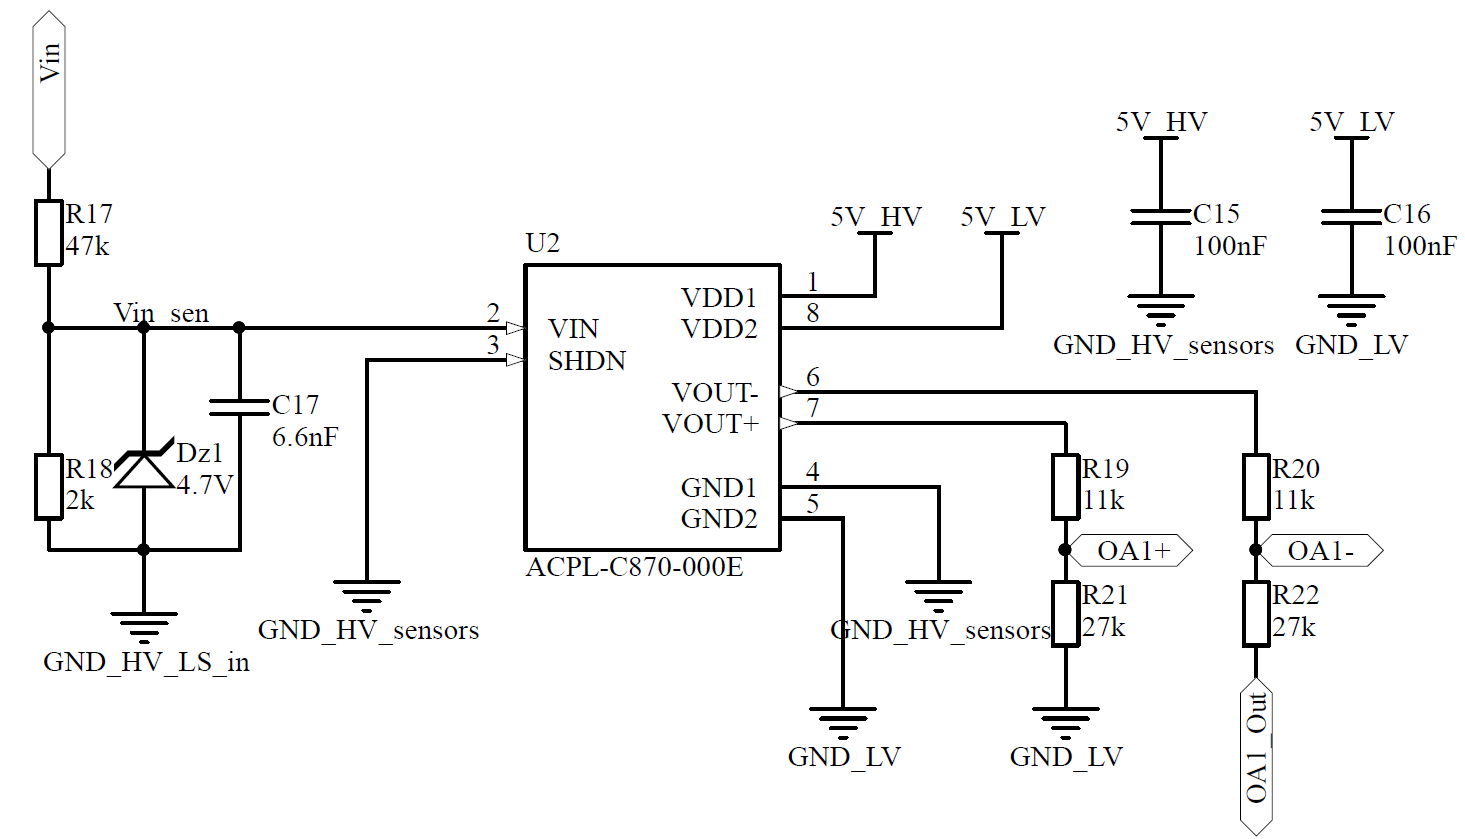
\includegraphics[width=0.7\linewidth]{../Pictures/P1/Sensors/input_voltage_sensor.PNG}
		\caption{Input voltage sensor}
		\label{fig:input_voltage_sensor_circuit}
	\end{center}
\end{figure}

\subsection{Output voltage sensor}
The voltage sensor at the output is design by the same procedure as the input sensor. The voltage divider will designed such that the values of the amplifier can be reused.

\subsubsection{Voltage divider}
The maximum output voltage of the DC/DC converter will be $90V$, when only 4 PV-modules are used. To insert a safety margin if one converter fails, the maximum sensed voltage will be designed at $120V$.

The resistors will be sized by reusing equation \ref{voltage_divider_R17_in} and \ref{voltage_divider_R18_in}.
\begin{equation}
	R_{26} = \frac{V_{in,max}-V_{out}}{I} = \frac{120V-2V}{1mA} = 118k\Omega	
\end{equation}

\begin{equation} 
	V_{out} = V_{in,max} \cdot \frac{R_{27}}{R_{26}+R_{27}} \Rightarrow 2V = 120V \cdot \frac{R_{27}}{118k\Omega+R_{27}}
\end{equation}
\begin{center}
	$R_{27} = 2.03k\Omega$
\end{center}

To achieve these resistor values $R_{26} = 120k\Omega$ and $R_{27} = 2k\Omega$ have been chosen. 

\subsubsection{Filtering}
The filter will be design with the same corner frequency at $500Hz$, as for the input sensor.

The resistor of the filter will be $R_{26}$ in the voltage divider. The capacitor will be calculated as followed in equation \ref{voltage_sensor_out_filter_cap}:
\begin{equation} \label{voltage_sensor_out_filter_cap}
	C_{22} = \frac{1}{2\pi \cdot f_c \cdot R_{26}} = \frac{1}{2 \pi \cdot 500Hz \cdot 120k\Omega} = 2.6nF
\end{equation}

To achieve the capacitance $C_{22} = 3.3nF$ has been chosen. 

\subsubsection{The circuit}
The circuit regarding the input voltage measurement is shown at figure \ref{fig:output_voltage_sensor_circuit}. $V_{out}$ is the measured voltage from the converter output. The points $OA2_+$ and $OA2_-$ are connected to the non-inverting and inverting input of the amplifier respectively. $OA2_{out}$ is connected to the output of the amplifier. $C_{20}$ and $C_{21}$ are decoupling capacitors for the two supply voltages. 

\begin{figure}[H]
	\begin{center}
		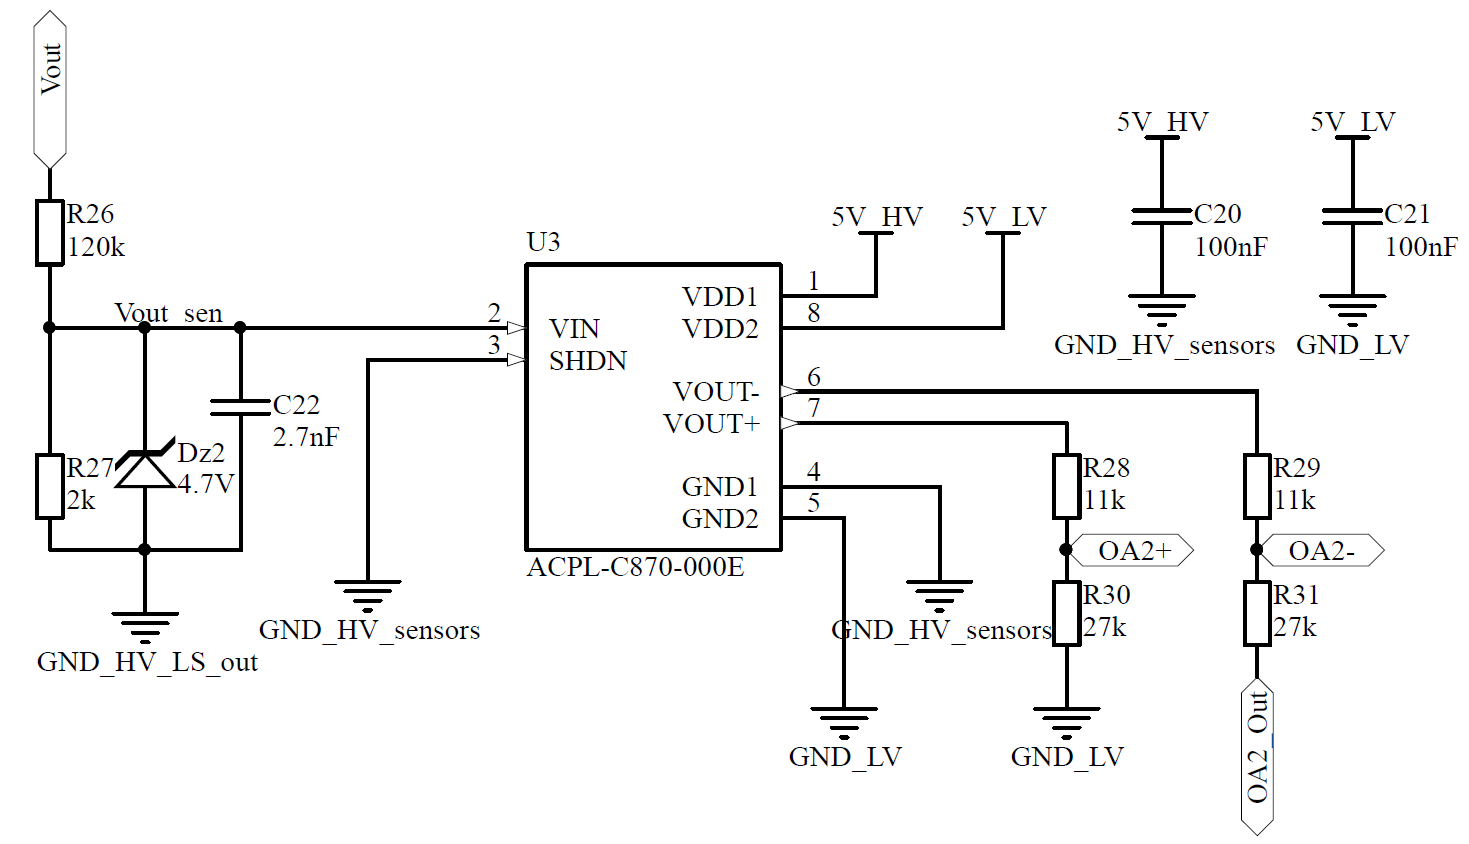
\includegraphics[width=0.7\linewidth]{../Pictures/P1/Sensors/output_voltage_sensor.PNG}
		\caption{Output voltage sensor}
		\label{fig:output_voltage_sensor_circuit}
	\end{center}
\end{figure}

%%% Current sensors %%%
\subsection{Current sensor} \label{current_sensor}

The current along with the voltage of the PV allows the system to perform power calculation, which is needed for the MPPT algorithm. The current will be measured in parallel with the inductor with a hall effect sensor. Placing it in series with the PV module would be the easiest approach for MPPT, but placing it in parallel with the inductor allows implementing a current controller for possible future use.

\begin{figure}[htbp]
	\begin{center}
		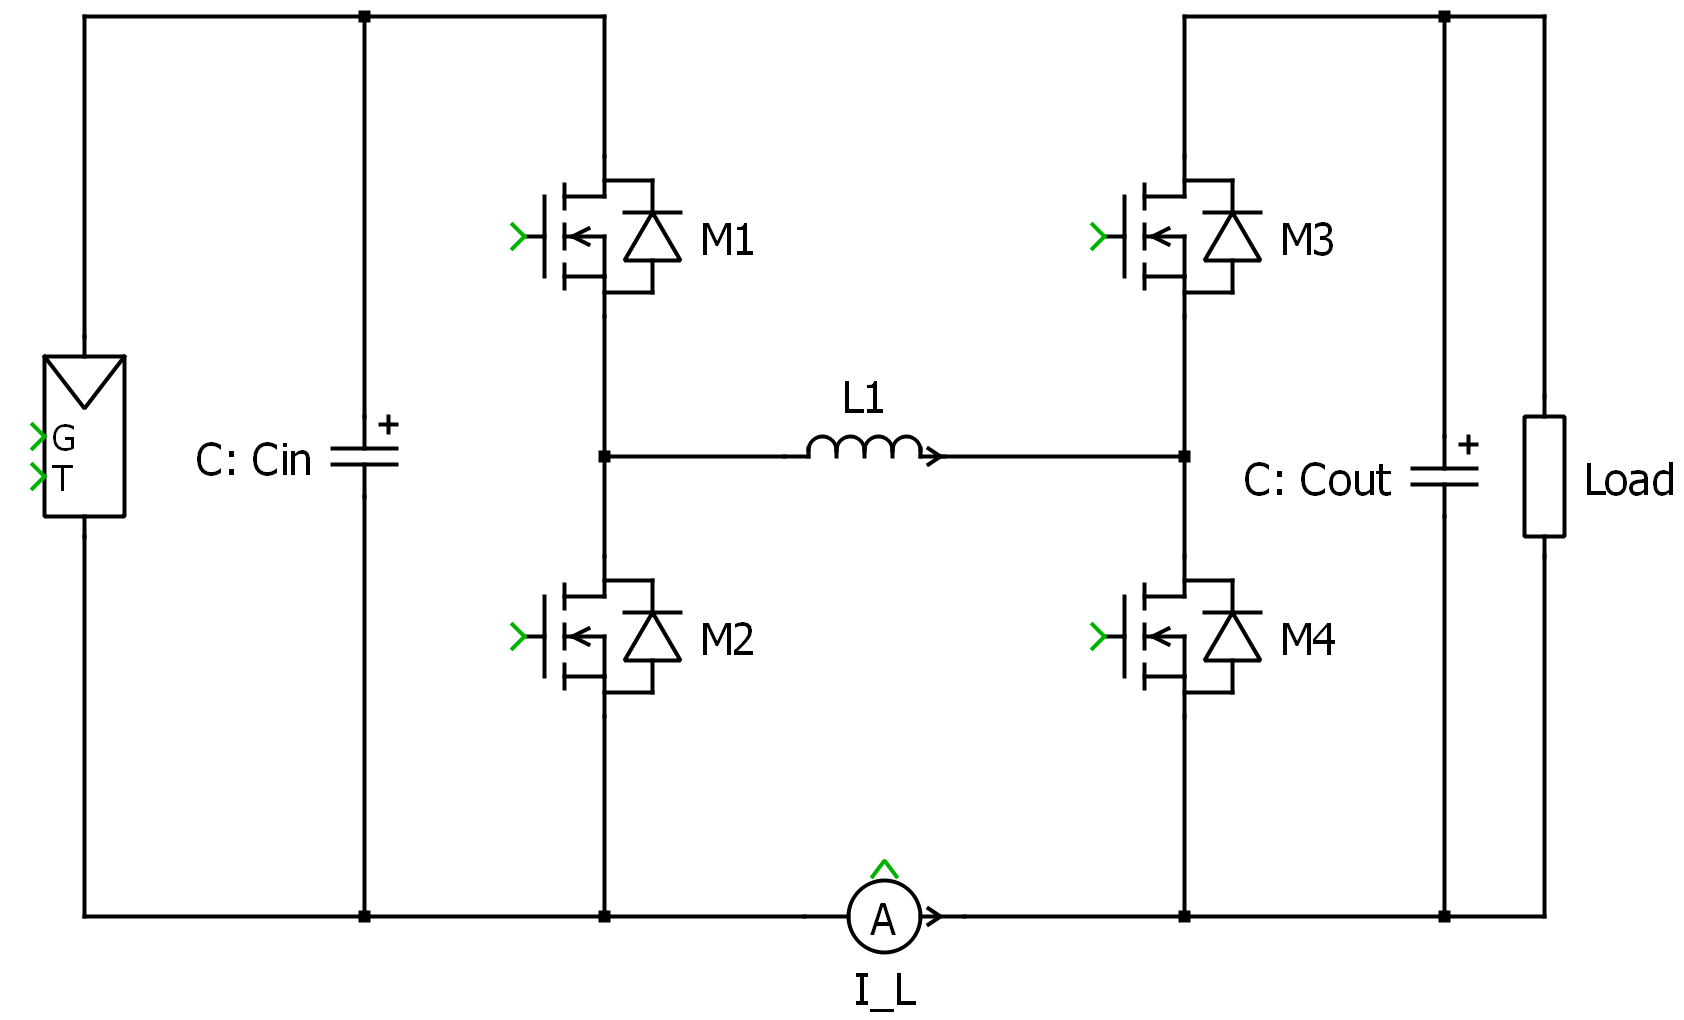
\includegraphics[width=0.4\textwidth]{../Pictures/current_sensor_placement.png}
		\caption{Current sensor placement.}
		\label{current_sensor_placement}
	\end{center}	
\end{figure}

The sensor is a ACS723-20AB which is a Hall effect sensor. Its features might be found in table \ref{current_sensor_features}.

\begin{table}[htbp]
	\centering
	\begin{tabular}{|p{6cm}|>{\centering}p{8cm}|}
		\hline
		\rowcolor{lightgray}\multicolumn{2}{|l|}{ \textbf{Maximum ratings}} \\ \hline
		Supply voltage & 4.5-5.5 [V]  \tabularnewline \hline
		Gain & 100 [mV/A]  \tabularnewline \hline
		Input range & $\pm$20 [A]  \tabularnewline \hline
		\rowcolor{lightgray}\multicolumn{2}{|l|}{ \textbf{Other values of interest}} \\ \hline
		Bandwidth & 20 or 80 [kHz]  \tabularnewline \hline
		Package & SOIC8  \tabularnewline \hline
		
	\end{tabular}
	\caption{Current sensor figures of merit. \cite{current_sensor}}
	\label{current_sensor_features}
\end{table}

The output of the sensor is a voltage proportional to the current following the next equation:
 \todo[inline,color=green]{maybe the gain is 0.125, to be confirmed by test.}
\begin{equation} 
V_{current} = \frac{1}{10} \, i + 2.5
\end{equation}

In order to ease the task of the control, the signals are filtered by hardware. The current will be used by the MPPT, which frequency is $100 Hz$ \todo{check final implementation}. The sensor output is filtered by a LPF which cut-off frequency is $500 Hz$. The cut-off frequency has been calculated by a hundredth of the switching frequency, which is $50 kHz$. Also the current might be used in the current controller, this signal will be filtered at $80 KHz$ in order to remove high frequency noise, this cut-off frequency was selected as it is the sensor's bandwidth. The filters are first order low-pass filters implemented with a resistor in series with a capacitor.\todo{has the current control been implemented? was enough this filtering?}

In order to calculate the current from the PV module, the converter working mode will have to be taken into account. Assuming continuous conduction mode, the average PV current is:


\begin{equation} 
	Buck \; mode \rightarrow \overline{I_{in}} = i_{measured} \cdot \delta
\end{equation}
\begin{equation} 
Boost \; mode \rightarrow \overline{I_{in}} = i_{measured} \cdot
\end{equation}
\begin{equation} 
Buck-Boost \; mode \rightarrow \overline{I_{in}} = i_{measured} \cdot \delta
\end{equation}

The IC has been placed far from the inductor in order to avoid undesired magnetic flux.

 
